% !TEX root =  ../geospatial-video.tex

\section{Domain-Specific Language}
\begin{figure*}[t]
    \centering
    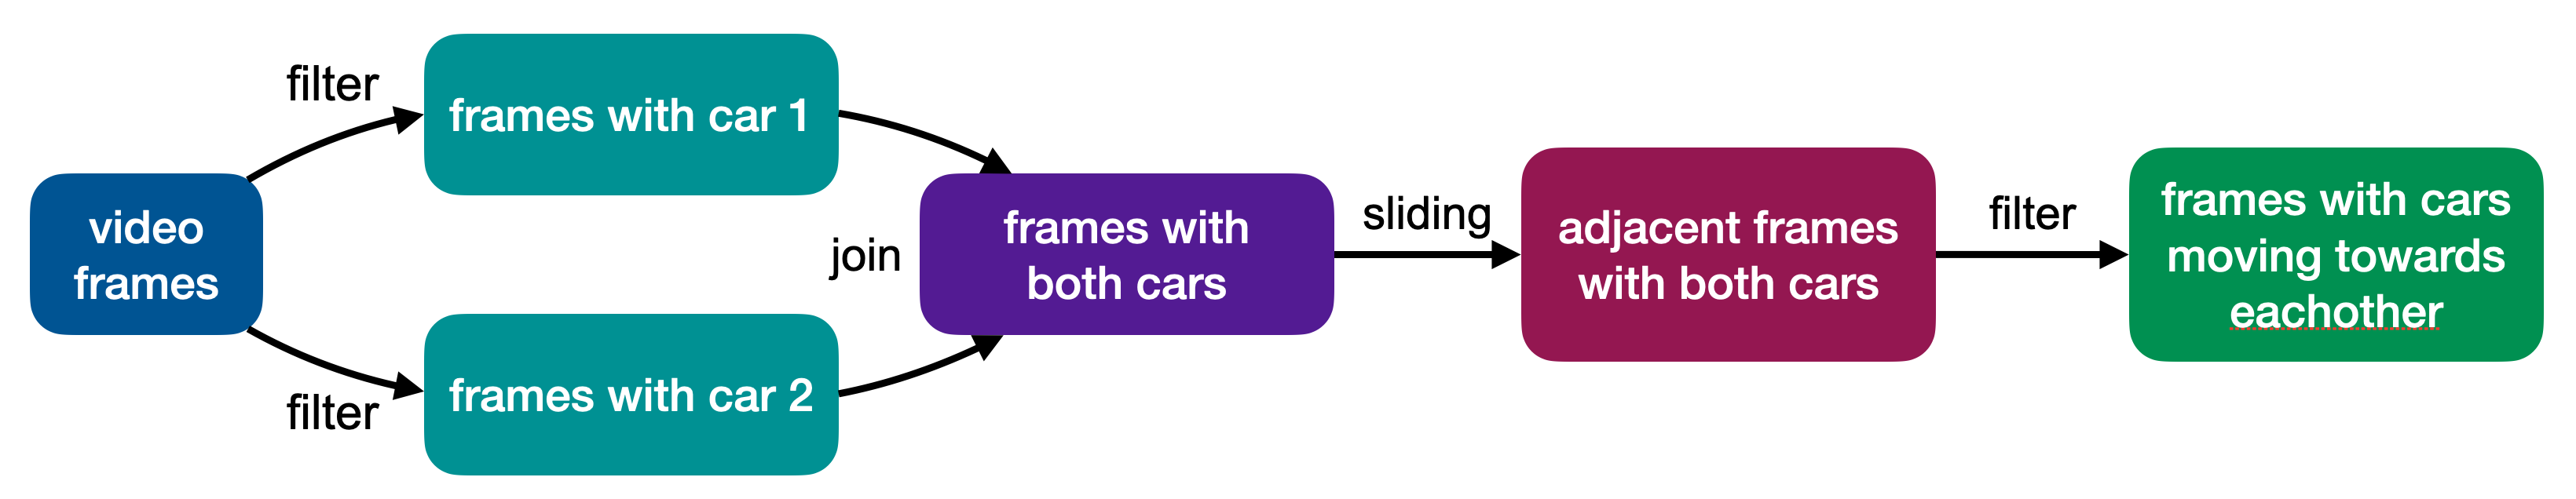
\includegraphics[width=\textwidth]{figures/declarative-dataflow.png}
    \caption{An example of a dataflow users can construct for a complex query.}
    \label{fig:declarative_dataflow}
\end{figure*}
\todo{to focus: \\
- by-frames operations: as a response to Lisa's use case where we need to scope the output video to the only interesting parts of each videos. \\
- by-frames <--> by-instances: as a response to Yousef's comments to allow the language to express more queries
}

To address the pain points we noticed in our user interviews, we chose to design a new language for describing queries over geospatial video data as a domain-specific language embedded in Python. Instead of building a new language from scratch, which would require designing a new syntax and editor integrations that users would have to learn about, we are able to inherit the large ecosystem of existing tooling around Python. Furthermore, some potential users of our system are already familiar with Python, which makes it further easier to integrate into existing pipelines.

\subsection{Design Guidelines}
There are three key factors constraining the design of our language: incremental query creation, support for using the language through a graphical user interface, and supporting queries that combine predicates over time and space. Before we dive into how we design the language around these constraints, let us walk through how we derived the factors based on our user-studies and their consequences on the space of language designs.

\subsubsection{Incremental Queries}
Across the interviews, a key pattern that stuck out was the process by which the participants would identify portions of video that were of interest---either by manual scrubbing through video files or the creation of queries. Rather than define the end-to-end query, the participants would start with a coarse grained search, looking for portions of the video that are likely to have the information they are looking for. Across these sections, the participants would then refine their search/query by playing back the video in real-time or querying individual frames in more detail.

Our insight from this observation was that users of video query languages will want to develop the query incrementally, where they can start with a query that identifies sections of the video with general patterns related to their specific goal (such as the presence of multiple cars in the same frame) and iteratively refine it to identify the specific scenario (such as cars moving towards each other) while receiving feedback from the query engine.

Supporting incremental query creation places significant constraints on the design of the language since the language must offer modular APIs to support users adjusting their query pipelines over time and must also have a performant runtime that can execute updated queries efficiently. Furthermore, it requires us to ascribe meaning to intermediate steps of a query, including complex concepts such as windows over time or groups of objects, so that users can see the results of each component of their pipeline.

\subsubsection{Graphical User Interface}
Based on our interview with Lisa Pickoff-White, who works on data journalism but primarily uses manual scrubbing methods to query videos rather than writing code, we identified that a key feature to make our language useful is offering a graphical interface for constructing programs for users who are not comfortable with text languages. At the same time, however, we want to support a lower-level Python API for constructing queries that expert users such as Yousef would be more comfortable using.

To support this graphical interface, we decided to design it as a layer on top of the Python API with mappings from each concept in the low-level to features in the interface. This architecture means that the low-level API should be strongly typed, since types in the API can be used to constrain the types of programs in the graphical interface to those that are correct by construction. Furthermore, it requires us to include several built-in APIs for common scenarios to reduce the overhead of describing various queries.

\subsubsection{Queries over Time and Space}
Finally, we observed in both interviews that queries over video data often require repeatedly moving between the axis of time and detected objects, something that existing query systems do not support. For a concrete example, consider an query over autonomous vehicle data that is looking for collisions. We want to find chunks of the video where two cars are moving to each other, but this requires predicates that both reason about multiple frames together and multiple objects together. After a user writes a query to identify cars, they will need to identify \emph{frames} with multiple cares, and then process windows of frames to check if the detected objects are moving towards each other.

Queries like this are difficult or impossible to describe with existing query languages, which either focus exclusively on time or objects as the primary axis being queried over. We aim to address this in our design by providing APIs that mix these two concepts together, enabling queries such as filtering over the properties of objects in windows of time. This requires us to extend the data model, as we discussed in the previous section, and also provide APIs for switching between the frame and instance views of video data.

\subsection{Language Design}
With these design goals, we decided to develop a DSL based on declarative and functional programming principles. Rather than writing out queries as imperative statements that mutate data, have unclear dependencies, and use hard-to-optimize control constructs, this approach allows us to optimize and execute the queries users write from a global perspective. By modeling queries as dataflows, such as the example in Figure~\ref{fig:declarative_dataflow}, our language can also provide high-quality intermediate feedback since every intermediate node can be mapped to output samples. Finally, the declarative approach makes it simpler to build a graphical interface, since the dataflow model corresponds to a natural visual model of connecting primitive operations with dependencies.

Our DSL consists of four core types corresponding to the elements of our data model: videos, frames, instances, and annotations. To develop dataflows over these structures, we then provide collection types wrapping these elements, which represent nodes that will process incoming streams of video data. In the time domain, we also include a collection type that captures groups of frames rather than just individual elements, which is useful when performing tasks like tracking the motion of an object over a window of time.

To create complex queries, users can develop a dataflow pipeline by repeatedly transforming these collection types using functional operations. In addition to the classic transformations such as map, which transforms individual elements independent of each other, and filter, which applies a predicate to each element, we also include several operations specific to the domain of video data. First, we include the \texttt{join} operator, which allows a user to combine multiple collections by matching elements with a specific property. For example, users may join 


\shadaj{walk through functional APIs}

\shadaj{examples of code}

\shadaj{explain how to alternate between time/space}

% \subsection{Prototype Implementation}
% TODO?
